\section{Signature Extraction}

Each method of signature extraction described in this section has the fast
discrete curvelet transform at its heart. The curvelet transform has two main
parameters, that influence the result: The number of angles $N_{\theta}$ used
at the coarest scale and the number of scales $N_j$, which corresponds to the
number of concentric squares shown in \ref{fig:curvelet_discrete_tilings}.
Experiments conducted to determine the optimal values of these parameters have
shown that using more scales than 4 does not provide benefits that would
justify the increased amount of processing time. Furthermore, since the
coarsest scale is non-directional, as explained in section
\ref{sec:background_cct}, it is ignored in further computations.

The response image generated by the FDCT for each pair of scale and angle is
too large to be considered for the signature directly. Therefore the response
image $C_{s, \theta}$ for scale $s$ and angle $\theta$ is subdivided into $n^2$
equally sized grid cells $G_{s, \theta, x, y}$ with $x, y \in 1, 2, \dots, n$:
\begin{equation*}
    C_{s,\theta} =
    \begin{bmatrix}
        G_{s,\theta,1,1} & G_{s,\theta,1,2} & \cdots & G_{s,\theta,1,n} \\
        G_{s,\theta,2,1} & G_{s,\theta,2,2} & \cdots & G_{s,\theta,2,n} \\
        \vdots  & \vdots  & \ddots & \vdots  \\
        G_{s,\theta,n,1} & G_{s,\theta,n,2} & \cdots & G_{s,\theta,n,n} \\
    \end{bmatrix}
\end{equation*}
For each of these grid cells, the mean $\bar{C}_{s, \theta}$ is calculated:
\begin{align*}
    \bar{C}_{s,\theta} &=
    \begin{bmatrix}
        mean(G_{s,\theta,1,1}) & mean(G_{s,\theta,1,2}) & \cdots & mean(G_{s,\theta,1,n}) \\
        mean(G_{s,\theta,2,1}) & mean(G_{s,\theta,2,2}) & \cdots & mean(G_{s,\theta,2,n}) \\
        \vdots  & \vdots  & \ddots & \vdots  \\
        mean(G_{s,\theta,n,1}) & mean(G_{s,\theta,n,2}) & \cdots & mean(G_{s,\theta,n,n}) \\
    \end{bmatrix} \\
    &=
    \begin{bmatrix}
        \bar{c}_{s,\theta,1,1} & \bar{c}_{s,\theta,1,2} & \cdots & \bar{c}_{s,\theta,1,n} \\
        \bar{c}_{s,\theta,2,1} & \bar{c}_{s,\theta,2,2} & \cdots & \bar{c}_{s,\theta,2,n} \\
        \vdots  & \vdots  & \ddots & \vdots  \\
        \bar{c}_{s,\theta,n,1} & \bar{c}_{s,\theta,n,2} & \cdots & \bar{c}_{s,\theta,n,n} \\
    \end{bmatrix}
\end{align*}

\begin{figure}[h]
    \centering
    \subfloat[Curvelet coefficients]{%
        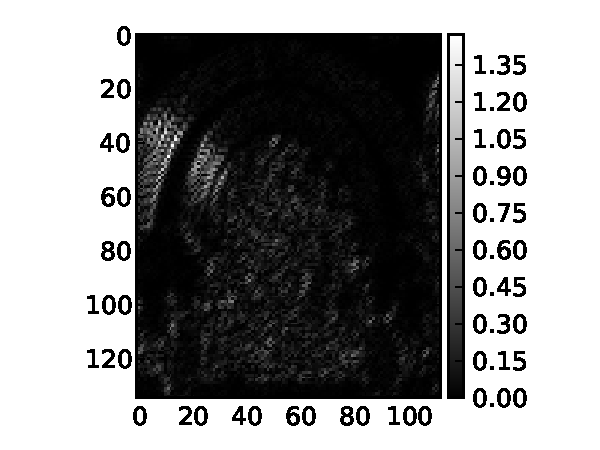
\includegraphics[width=0.45\textwidth]{signature_example_curvelet}%
        \label{fig:signature_example_curvelet}%
    }
    \quad
    \subfloat[Means on $8 \times 8$ grid]{%
        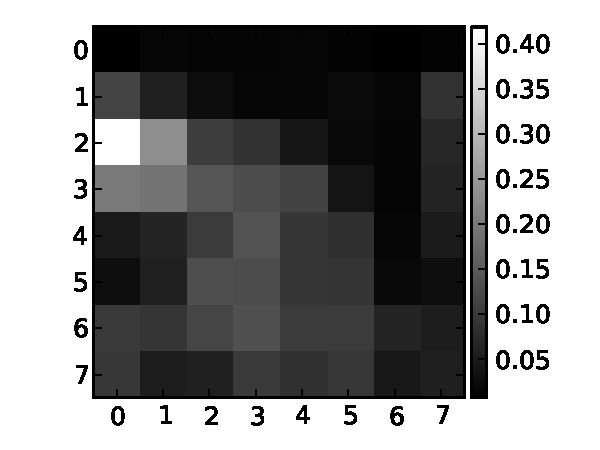
\includegraphics[width=0.45\textwidth]{signature_example_curvelet_means}%
        \label{fig:signature_example_curvelet_means}%
    }
    \caption[Curvelet coefficients and means]{
        The curvelet coefficients for a specific scale and angle can be seen in
        \subref{fig:signature_example_curvelet}. In
        \subref{fig:signature_example_curvelet_means} the response image has
        been subdivided into $8 \times 8$ cells and the mean value of each cell
        are shown.
    }
    \label{fig:input_examples}
\end{figure}


\subsection{Global Features}

\paragraph{MEAN}

The global approach to signature extraction simply takes the family of matrices
$\bar{C}_{s, \theta}$ and concatenates them as the image signature.

\subsection{Local Features}

The local feature extraction methods used here follow the bag-of-features
approach, that aims to represent an image using a set of local feature
descriptions or "visual words" similar to what was described in
\autocite{sivic_video_2003}. The exact way to extract the words will be
detailed towards the end of this section.

The set of visual words extracted from the images are diverse and hard to
compare. In order to create meaningful image signatures from these words, the
whole set is condensed into a dictionary using k-means clustering. As already
discussed in \ref{sec:anatomy_clustering}, the goal thereof is to derive a
dictionary of predefined size that contains the visual words corresponding to
the most discriminating features of the images in the image database. A
universally optimal size for the codebook does not seem to exist, as Nowak et
al.\ \autocite{nowak_sampling_2006} observe an increase in accuracy up to 1000
words, but overfitting for some sampling algorithms beyond that. At the same
time \autocite{yang_evaluating_2007} report optimal sizes of 20000 to 80000
depending on the image database. In \autocite{eitz_sketch-based_2010} a size of
1000 visual words was found optimal for sketches.

\paragraph{PMEAN}

Continuing from the set of matrices $\bar{C}_{s, \theta}$, this algorithm
densly samples each matrix by sliding a window of size $m \times m, m < n$
across it. This results in $n - m + 1$ parts $\bar{W}_{s, \theta, u, v}$ with
$u, v \in 1, \dots, n - m + 1$:
\begin{equation*}
    \bar{W}_{s,\theta,u,v} =
    \begin{bmatrix}
        \bar{c}_{s,\theta,u,v} & \bar{c}_{s,\theta,u,v+1} & \cdots & \bar{c}_{s,\theta,u,v+m} \\
        \bar{c}_{s,\theta,u+1,v} & \bar{c}_{s,\theta,u+1,v+1} & \cdots & \bar{c}_{s,\theta,u+1,v+m} \\
        \vdots  & \vdots  & \ddots & \vdots  \\
        \bar{c}_{s,\theta,u+m,v} & \bar{c}_{s,\theta,u+m,v+1} & \cdots & \bar{c}_{s,\theta,u+m,v+m} \\
    \end{bmatrix}
\end{equation*}
For each pair $(u, v)$ these matrices are concatenated in a consistent way and
stored as the feature vectors of the image. That way, the algorithm derives $u
\cdot v$ vectors of length $N_s \cdot N_{\theta_s} \cdot m^2$ from each image,
where $N_{\theta_s}$ is the number of angles at the scale $s$.

\begin{figure}[h]
    \centering
    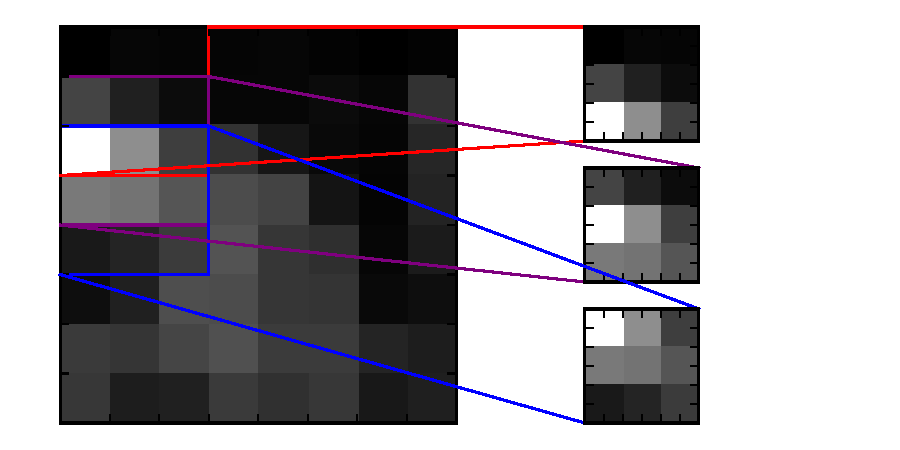
\includegraphics[width=0.9\textwidth]{signature_example_curvelet_patches}%
    \caption[Patches on a coefficient grid]{
        The mean coefficient grid $\bar{C}_{s, \theta}$ is densely sampled
        using a $3 \times 3$ window to produce $m^2$ patches per scale and
        angle.
    }
    \label{fig:patch_examples}
\end{figure}

\paragraph{PMEAN2}

In most parts, this variant is identical with the previously described PMEAN
algorithm with the exception of the final signature feature vectors. Instead of
concatenating all vectors $\bar{W}_{s, \theta, u, v}$, each scale is handled
separately. Therefore, each combination of $(u, v, s)$ produces a vector of
length $N_{\theta_s} \cdot m^2$.

\paragraph{Sampling}

Both of the feature vector extraction methods described above use dense,
overlapping sampling of a grid of mean values. By using $m \times m$ windows,
the small-scale spatial relationship between features can be captured. The
overlap helps to avoid misinterpretation of features on grid boundaries that
would occur with dense, non-overlapping sampling. Evaluations by Nowak et al.\
\autocite{nowak_sampling_2006} have shown that random sampling, which dense
sampling is a special case of, outperforms keypoint-based sampling for large
enough numbers of samples. Dense sampling on grids has previously been
successfully used by Lazebnik in \autocite{lazebnik_beyond_2006} and
\autocite{lazebnik_spatial_2009}. The R-HOG descriptor
\autocite{dalal_histograms_2005} also uses a dense grid for sampling with
overlapping windows to improve matching performance.
